\documentclass{beamer}

\usepackage{lmodern}

\usepackage{listings}

\usepackage[T2A]{fontenc}
\usepackage[utf8]{inputenc}

\usetheme{Madrid}
\usecolortheme{beaver}

\title[Erlang]{Исследование эффективности реализации\\некоторых структур данных на языке Erlang}
\subtitle[ПМИ]{Прикладная математика и информатика}

\author[Быцюк В.В.]{Быцюк Владислав Вячеславович}
\date[Брагилевский В.Н.]{Научный руководитель:\\старший преподаватель Брагилевский В.Н.}

\begin{document}
	\setbeamertemplate{caption}{\raggedright\insertcaption\par}

	% Титульный лист
	\begin{frame}
		\titlepage
	\end{frame}

	% Постановка задачи
	\begin{frame}{\LARGE \textbf{Постановка задачи}}
		\begin{itemize}
			\item Реализовать структуру данных <<упорядоченное множество>> на языке программирования Erlang.
			\item Сравнить время выполнения основных операций реализованной структуры данных с реализациями из модулей
			  	  ordsets и sets. 
		\end{itemize}
	\end{frame}
	
	
	% Основное содержание

	\begin{frame}[fragile]{\LARGE \textbf{Красно-черное дерево и Erlang}}
		\begin{figure}
			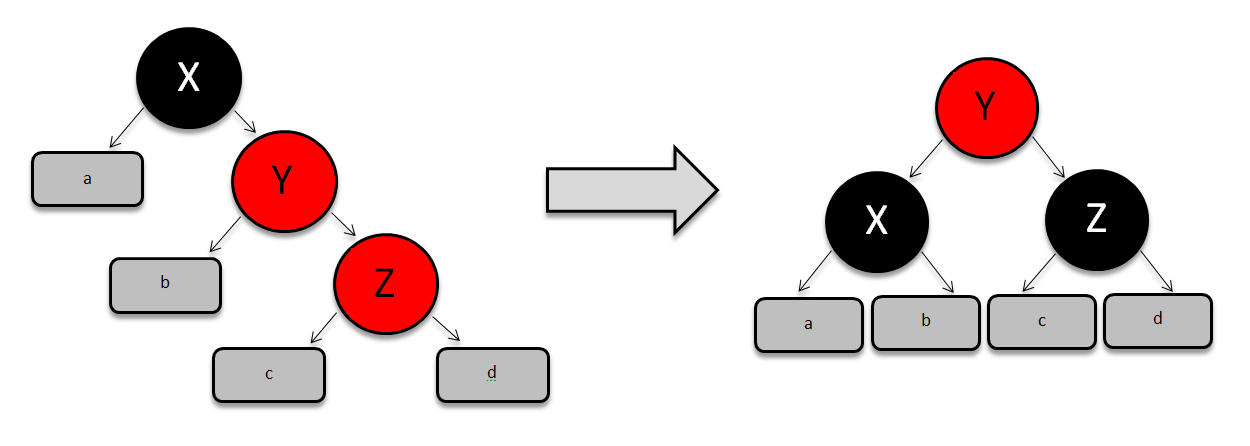
\includegraphics[scale=0.22]{img/clause_1.png}
		\end{figure}
		
		\pause
		
		\begin{block}{Реализация на Erlang}
			\begin{lstlisting}
balance({X, black, a, 
                   {Y, red, b, 
                            {Z, red, c, d}}}) ->   
	{Y, red, {X, black, a, b}, 
	         {Z, black, c, d}};		   
			\end{lstlisting}
		\end{block}	
	\end{frame}
	
	\begin{frame}{Сравнение времени выполнения операций вставки и удаления}
		\only<1>{
			\begin{figure}
				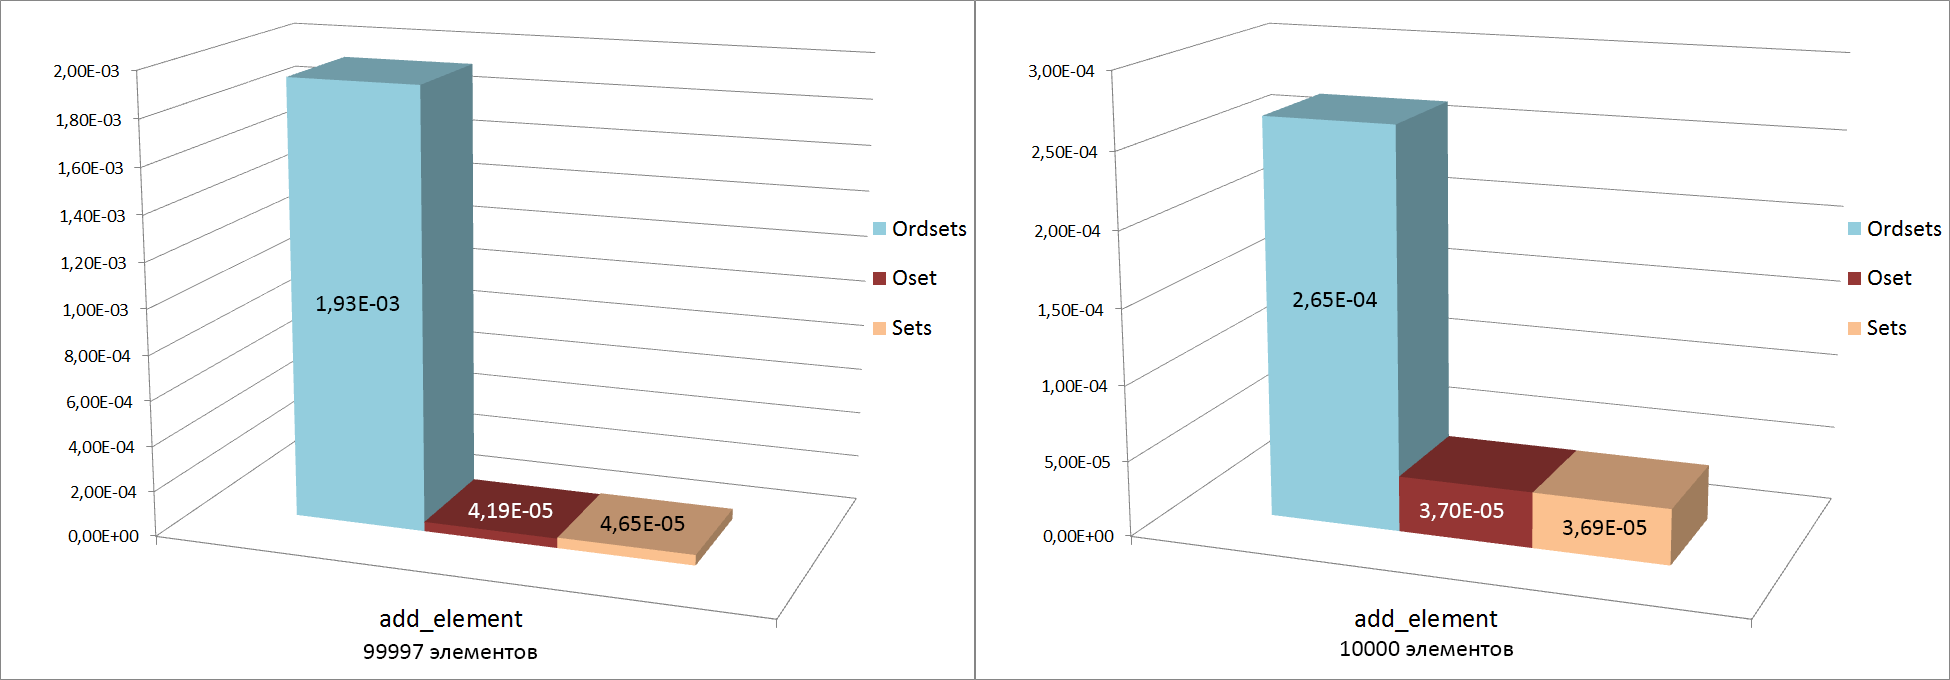
\includegraphics[scale=0.18]{img/histograms/add_element.png}
				\caption{Вставка}
			\end{figure}
		}
		
		\only<2>{
			\begin{figure}
				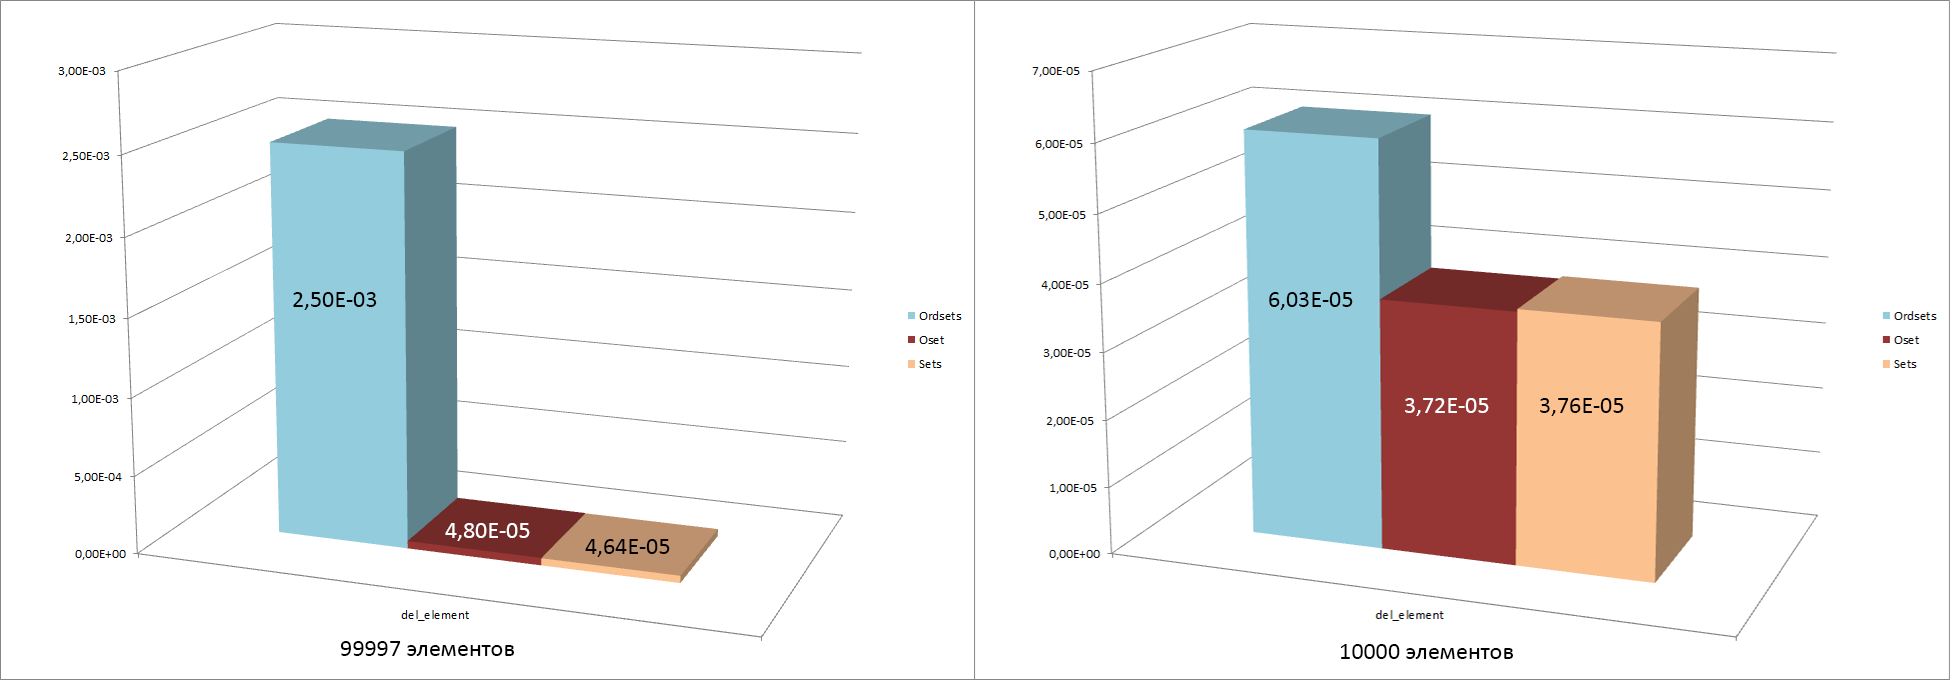
\includegraphics[scale=0.18]{img/histograms/del_element.png}
				\caption{Удаление}
			\end{figure}
		}
	\end{frame}
	
	
	\begin{frame}{Сравнение времени выполнения логических операций}
		\only<1>{
			\begin{figure}
				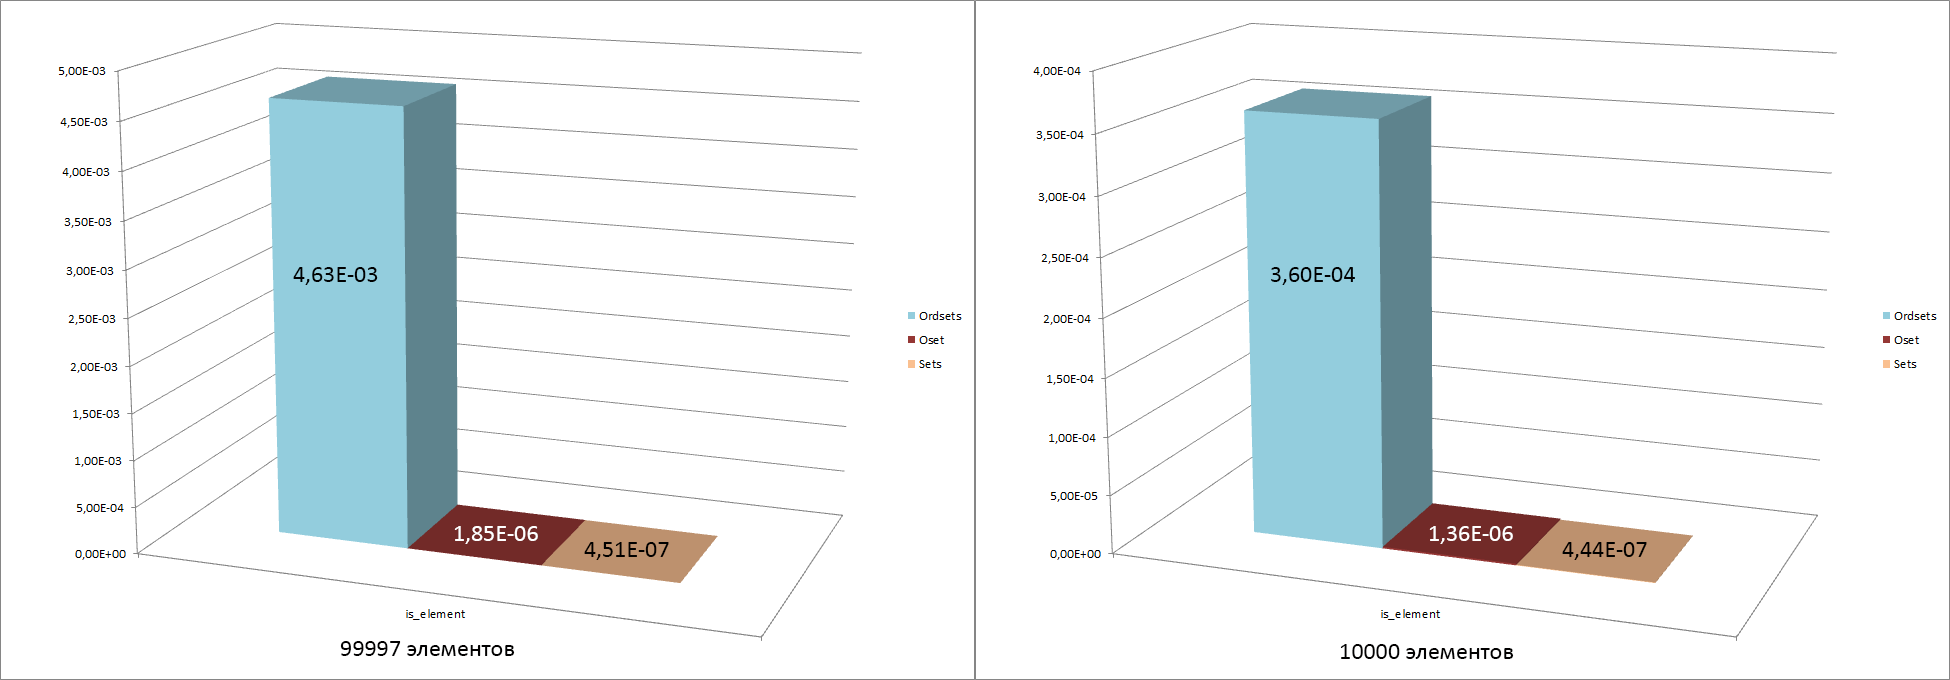
\includegraphics[scale=0.18]{img/histograms/is_element.png}
				\caption{Проверка на принадлежность элемента упорядоченному множеству}
			\end{figure}
		}
		
		\only<2>{
			\begin{figure}
				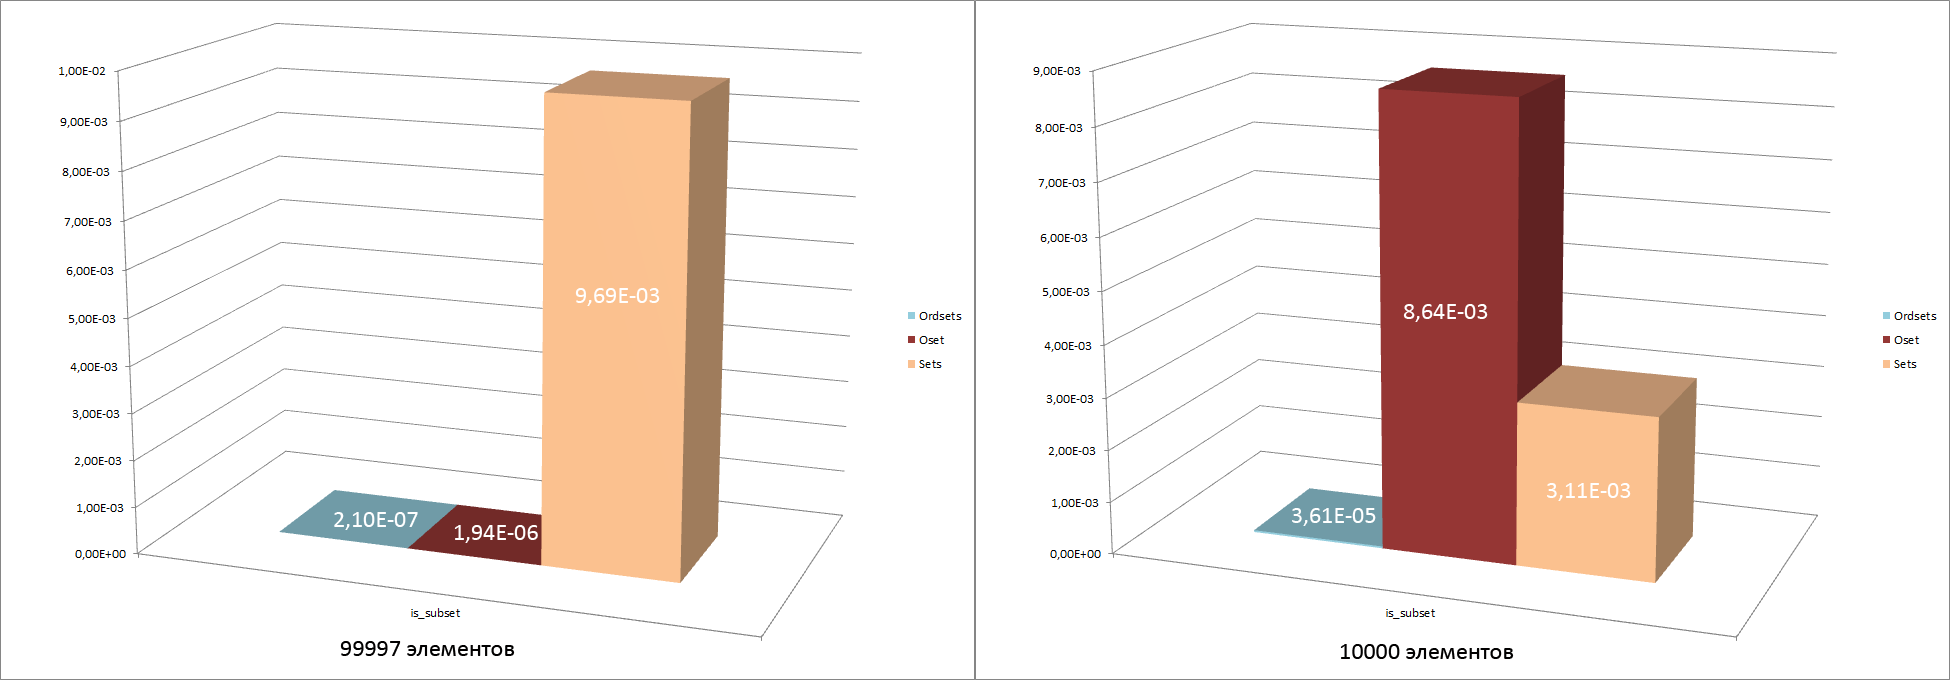
\includegraphics[scale=0.18]{img/histograms/is_subset.png}
				\caption{Проверка на то, является ли одно упорядоченное множество подмножеством другого}
			\end{figure}
		}
		
		\only<3>{
			\begin{figure}
				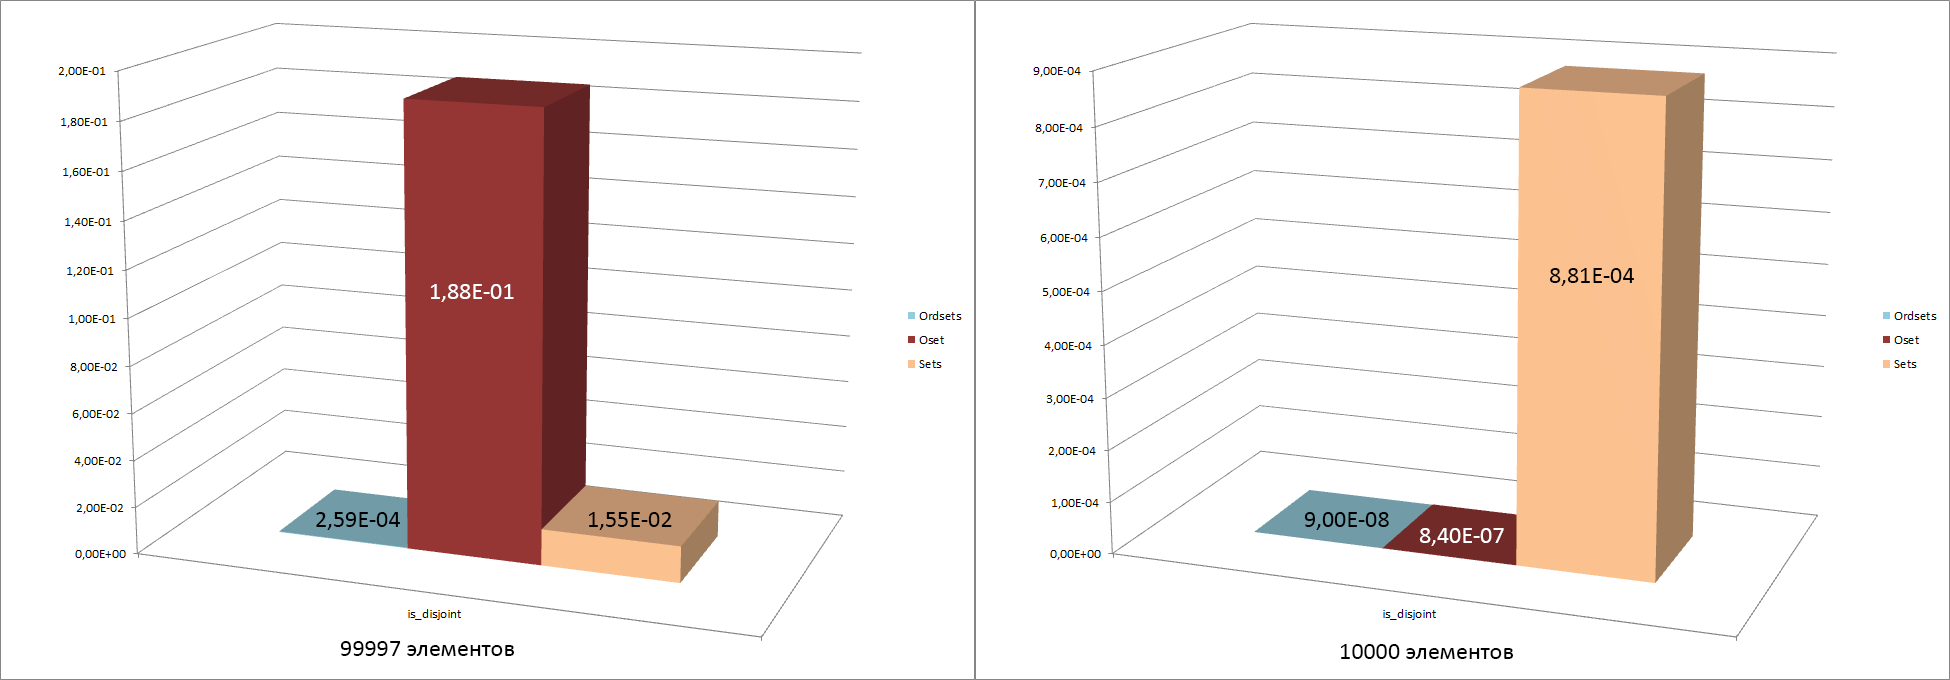
\includegraphics[scale=0.18]{img/histograms/is_disjoint.png}
				\caption{Проверка на непересекаемость двух упорядоченных множеств}
			\end{figure}
		}
	\end{frame}
	
	
	\begin{frame}{Сравнение времени выполнения перевод в список и обратно, свертки и фильтрации}
		\only<1>{
			\begin{figure}
				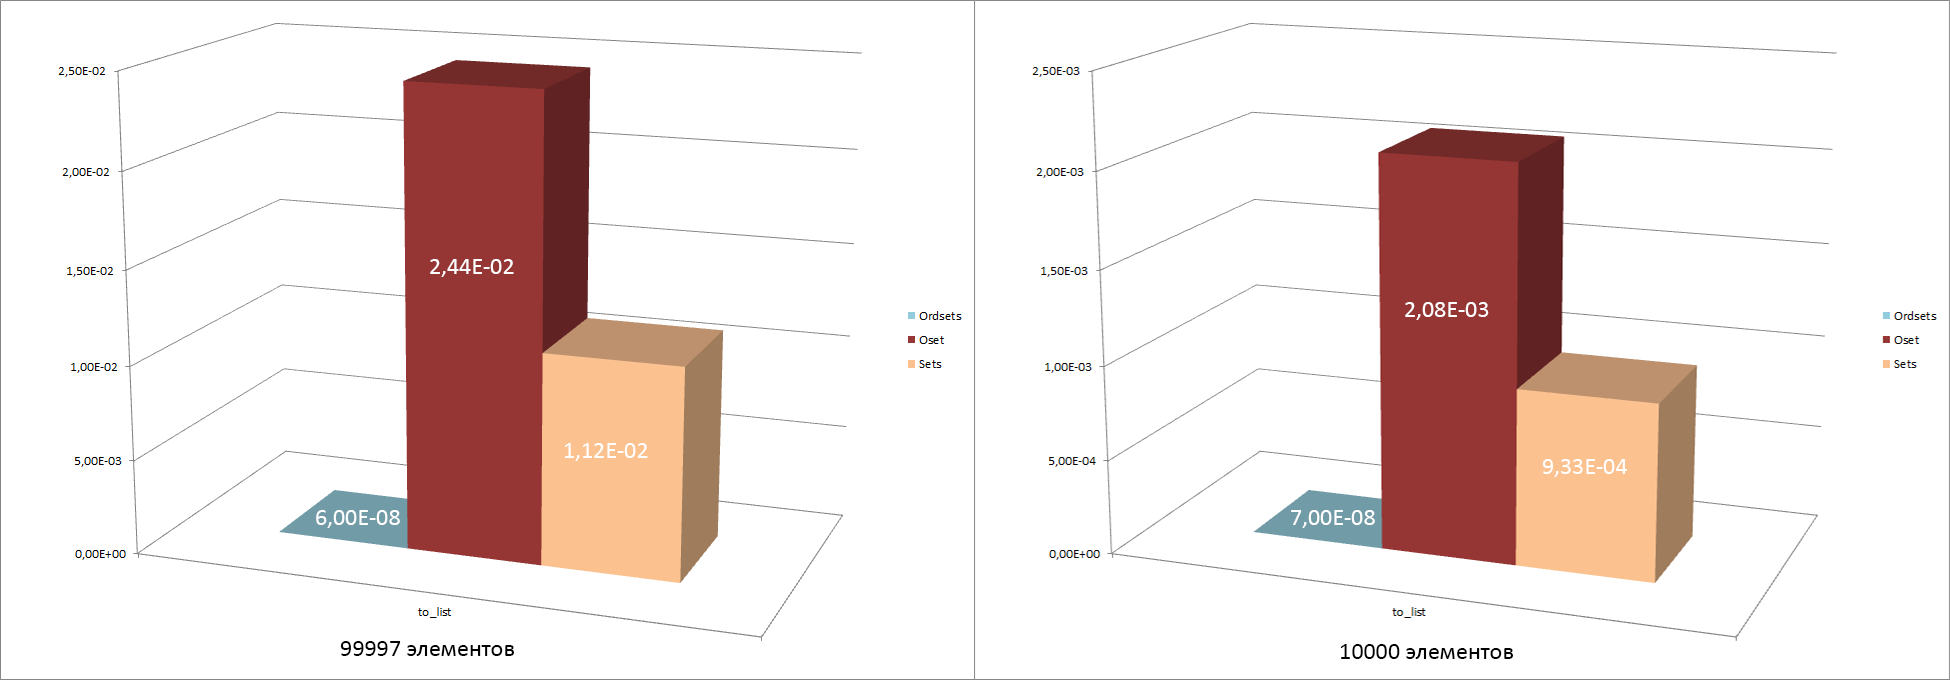
\includegraphics[scale=0.18]{img/histograms/to_list.png}
				\caption{Перевод упорядоченного множества в список}
			\end{figure}
		}
		
		\only<2>{
			\begin{figure}
				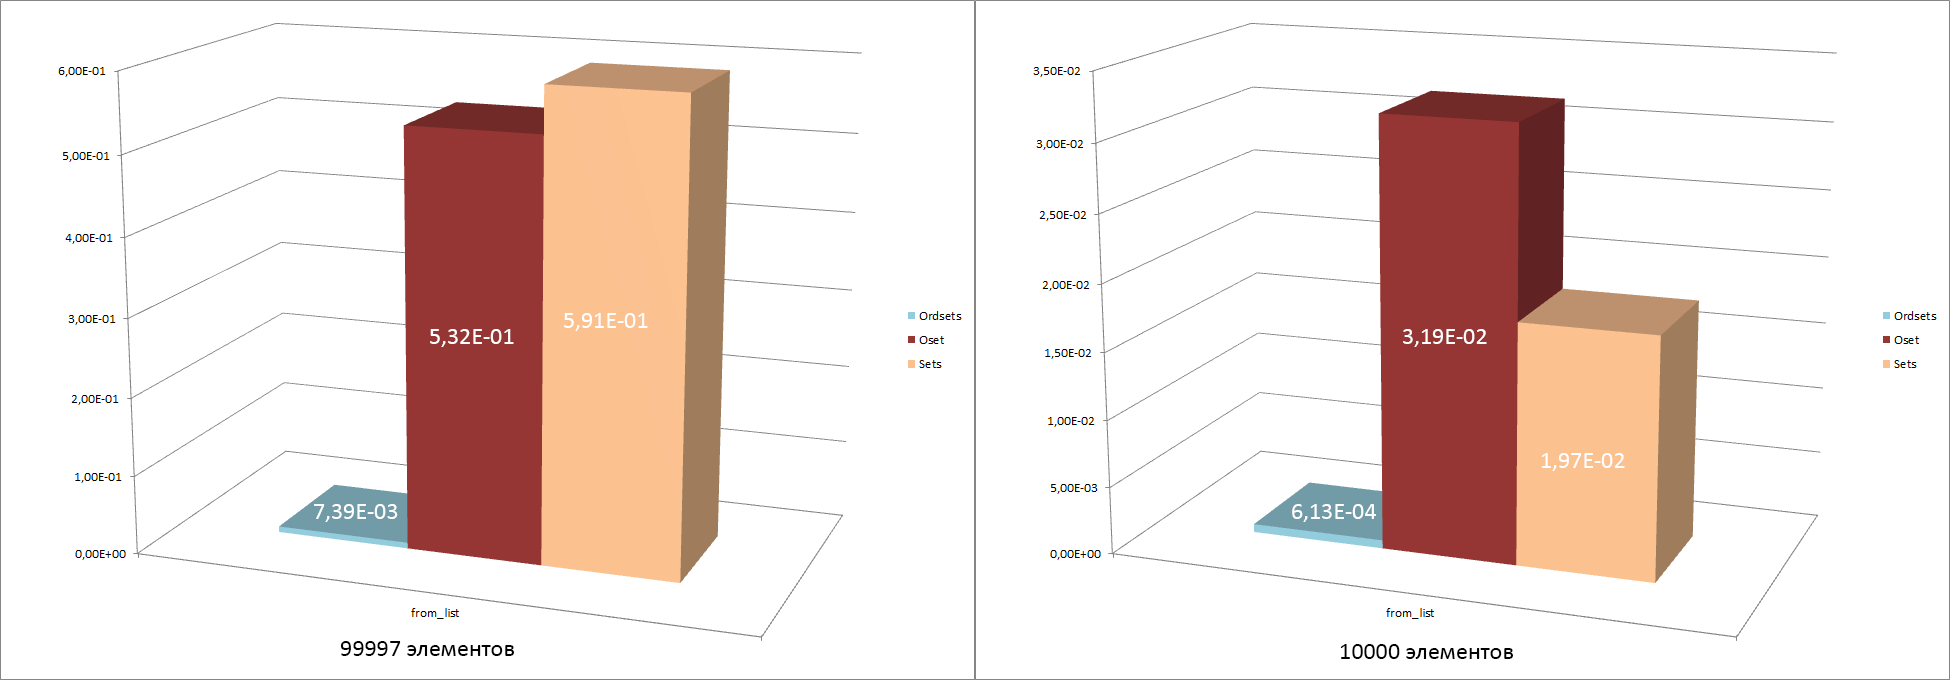
\includegraphics[scale=0.18]{img/histograms/from_list.png}
				\caption{Перевод списка в упорядоченное множество}
			\end{figure}
		}
		
		\only<3>{
			\begin{figure}
				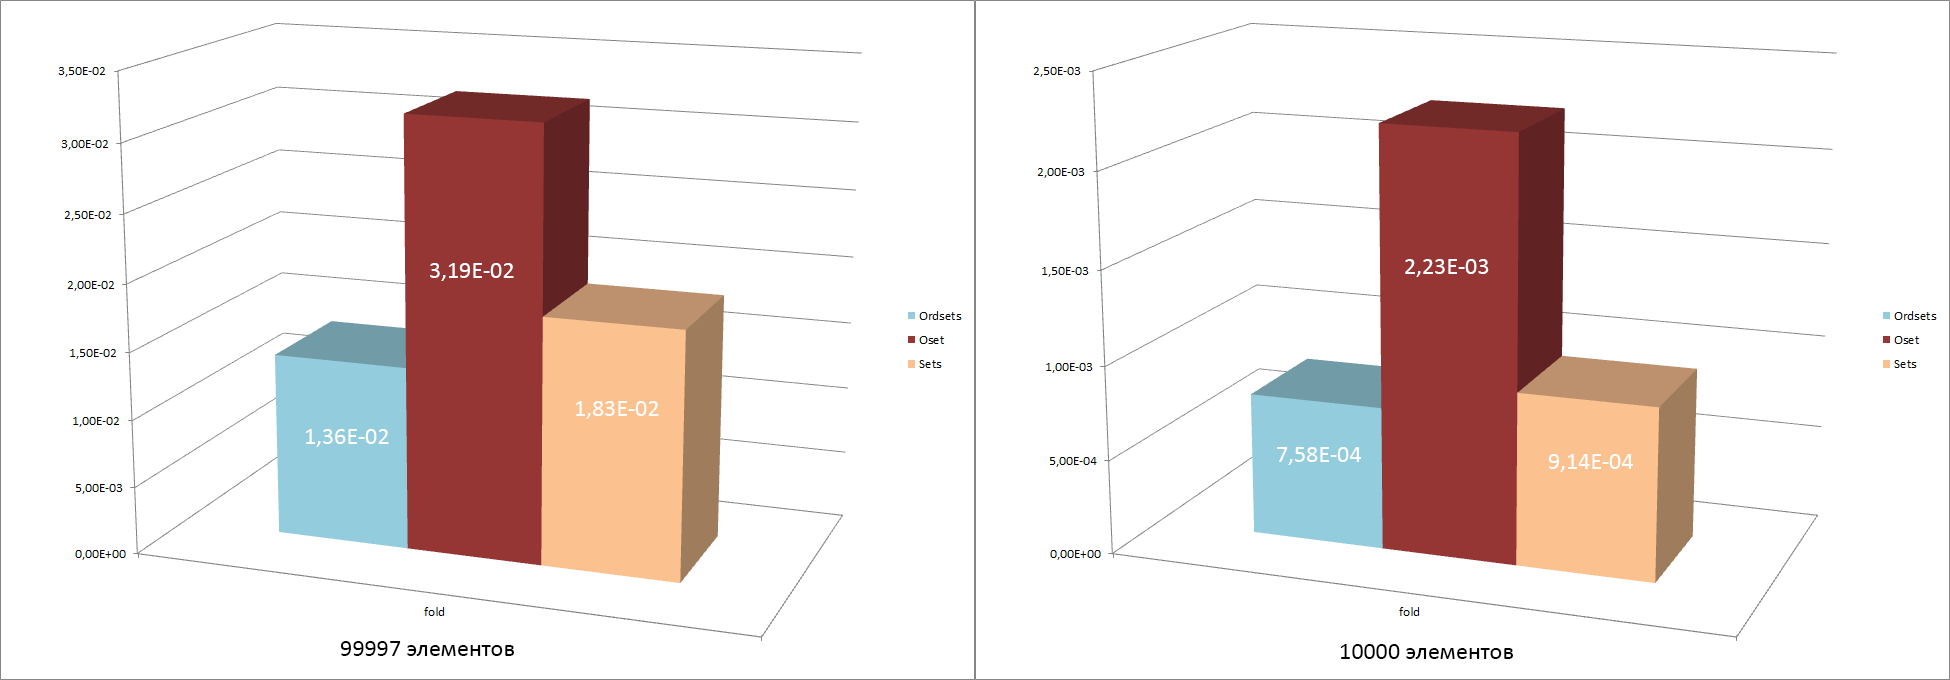
\includegraphics[scale=0.18]{img/histograms/fold.png}
				\caption{Свертка}
			\end{figure}
		}
		
		\only<4>{
			\begin{figure}
				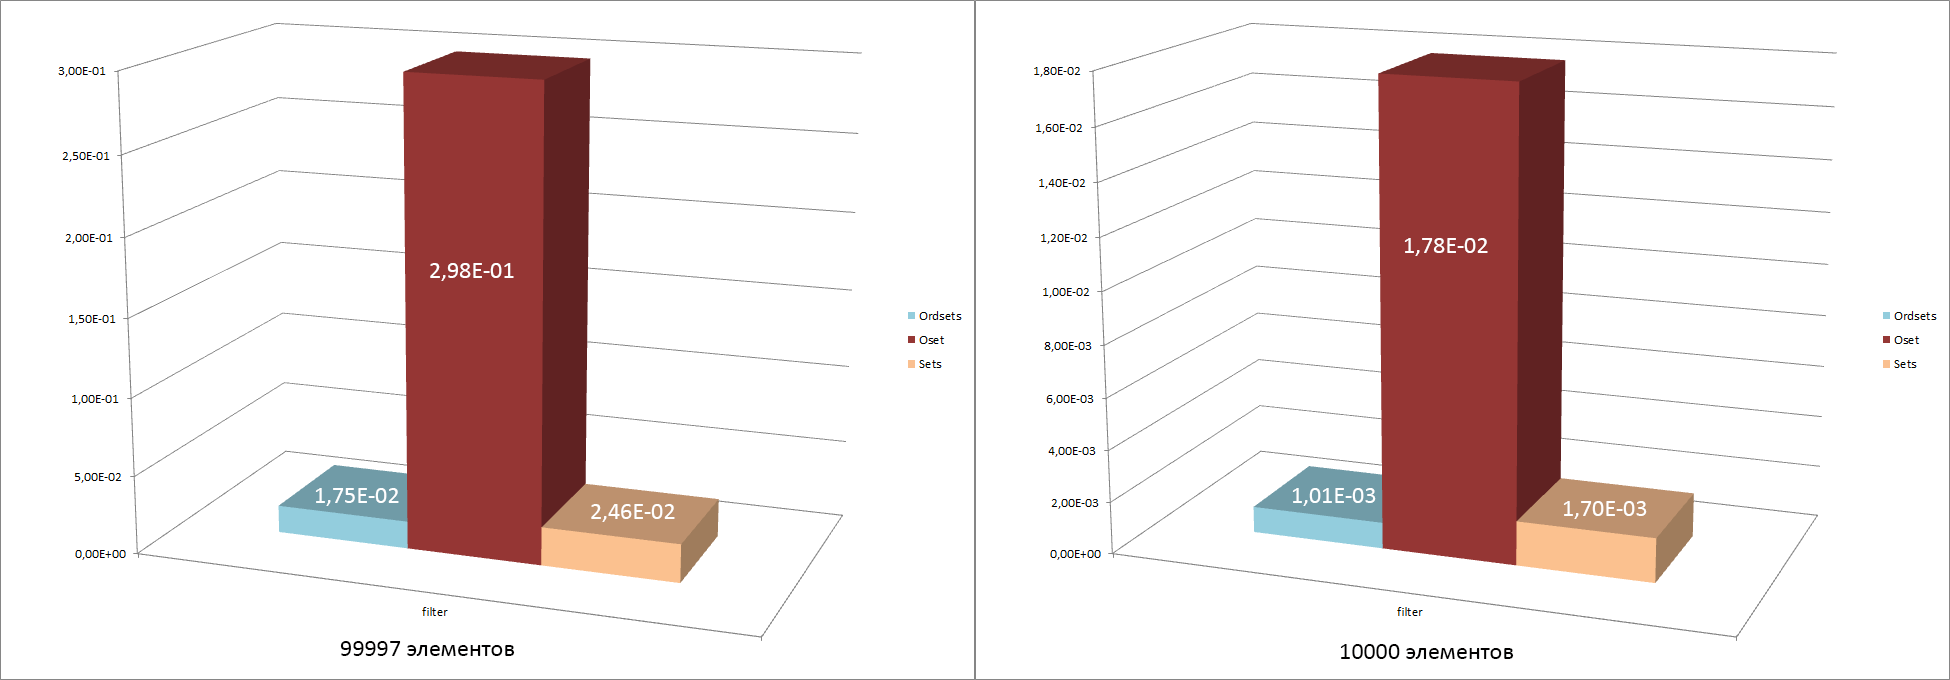
\includegraphics[scale=0.18]{img/histograms/filter.png}
				\caption{Фильтрация}
			\end{figure}
		}
	\end{frame}
	
	
	\begin{frame}{Сравнение времени выполнения операций объединения, пересечения, разности}
		\only<1>{
			\begin{figure}
				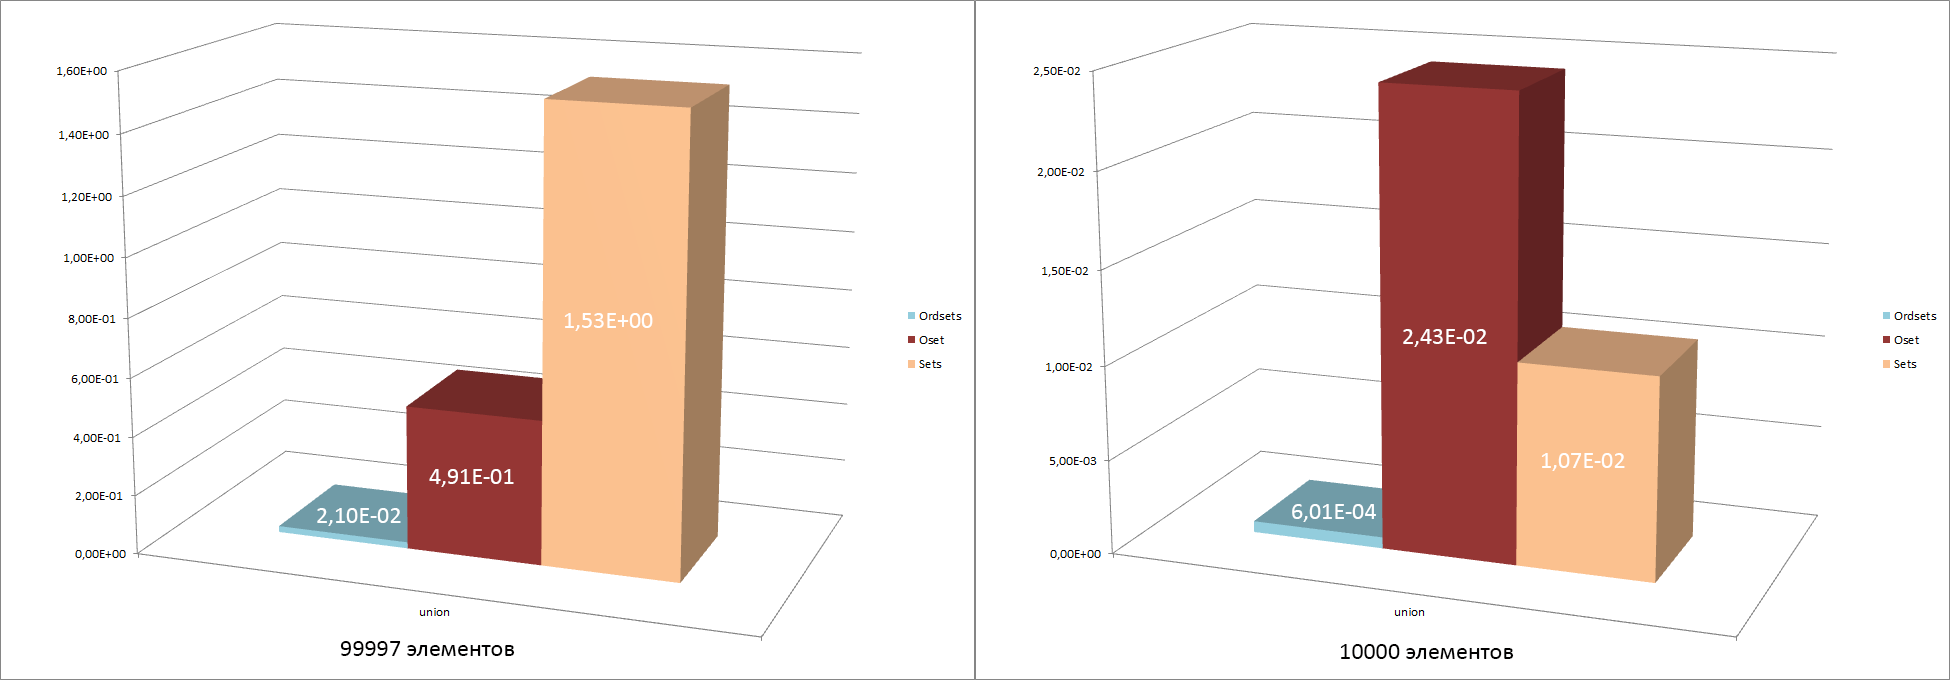
\includegraphics[scale=0.18]{img/histograms/union.png}
				\caption{Объединение}
			\end{figure}
		}
		
		\only<2>{
			\begin{figure}
				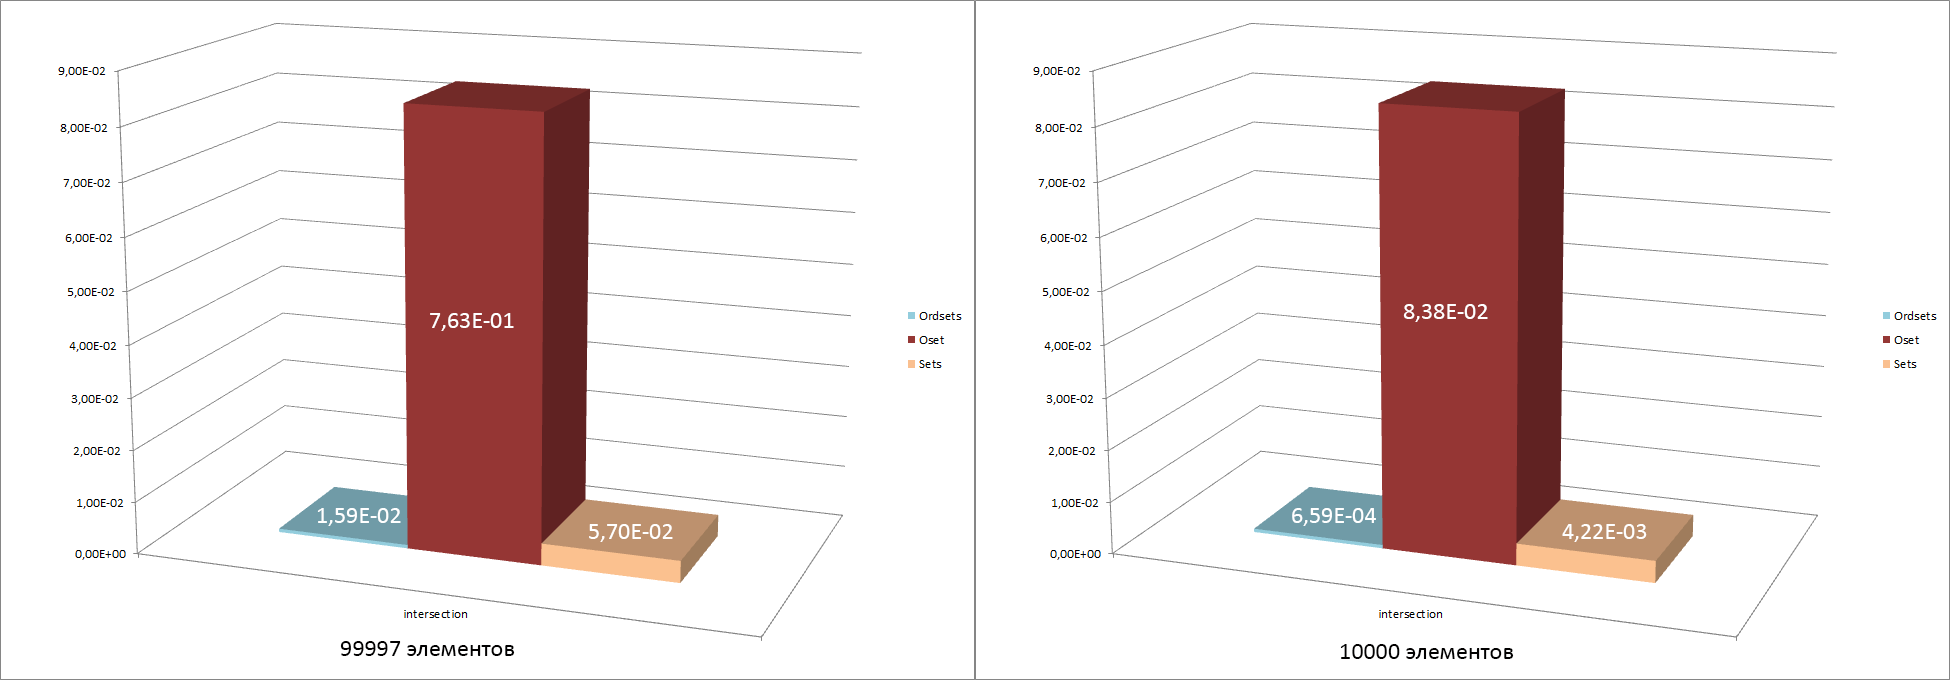
\includegraphics[scale=0.18]{img/histograms/intersection.png}
				\caption{Пересечение}
			\end{figure}
		}
		
		\only<3>{
			\begin{figure}
				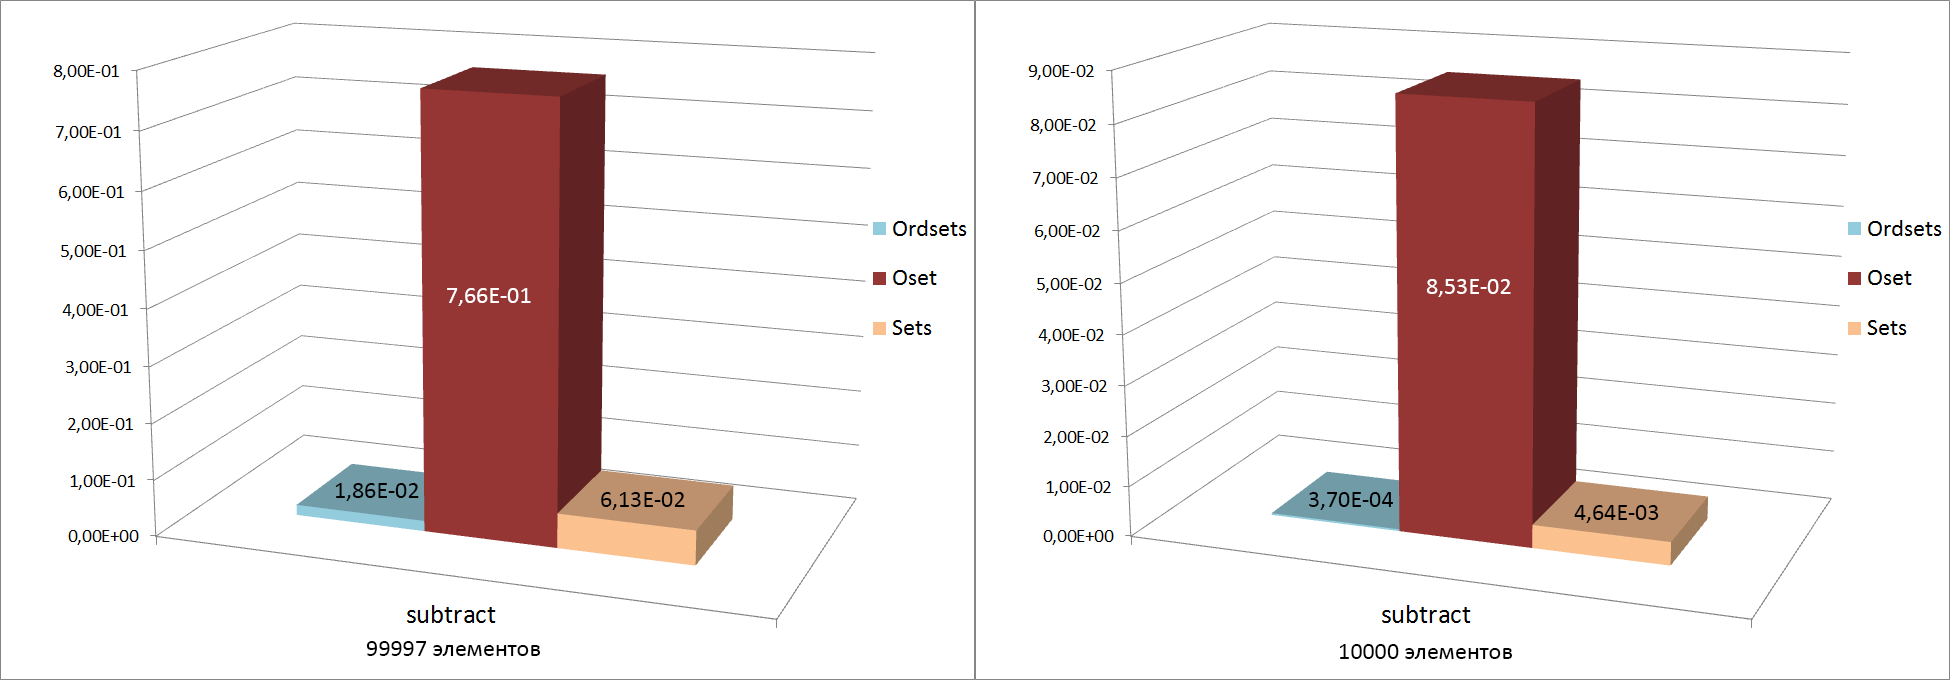
\includegraphics[scale=0.18]{img/histograms/subtract.png}
				\caption{Разность}
			\end{figure}
		}
	\end{frame}
	
	% Полученные результаты
	\begin{frame}{\LARGE \textbf{Полученные результаты}}
		\begin{itemize}
			\item Реализована структура данных <<упорядоченное множество>> на языке программирования Erlang.
			\item Проведено сравнение времени выполнения основных операций реализованной структуры данных с 
			      реализациями из модулей ordsets и sets. 
			\item Проанализированы результаты сравнения.
		\end{itemize}
	\end{frame}

\end{document}
